%\begin{flushleft}

\justifying
\chapter{\large INTRODUCTION}


\section{\normalsize BACKGROUND}


\hspace{1cm}In early days,it was much difficult for an individual to travel from one place to another.To reach a particular destination,while travelling at every turn he had to ask other person for the right path.This was quite time consuming and a reason for unnecessary extra fare at times if he go in a wrong way.\\
\hspace*{1cm}So to overcome these  problems and to reach the particular destination in lesser time with optimal path,this idea emerged.By using this HEPV algorithm,we can get the most optimum path between any two places.\\
\subsection{Basic Concepts}
\textbf{a) FlatGraph :}
\\
\hspace*{1cm}The graph of nodes and links where nodes represents the places
and links represents the path is called the flat graph.
\\
\textbf{b) Local Node :}
\\
\hspace*{1cm}The node which is present in only one fragment is called as 
	local node.
\\
\textbf{c) Border Node :}
\\
\hspace*{1cm}The node which is present in more than one fragment is called as border node.\\
\textbf{d) Fragments :}
\\
\hspace*{1cm}The flat graph is divided into smaller graphs to create a  
hierarchy of a graph are called as fragments.
\\
\hspace*{1cm}In our project we are taking flat graph of 30 nodes. The nodes are as follows:
\\

\hspace{0.5cm}1.	Pune  Station
\\ \hspace*{1cm}2.	Sanchetee  Hospital
\\ \hspace*{1cm}3.	Shivaji  Nagar
\\ \hspace*{1cm}4.	Manapa
\\ \hspace*{1cm}5.	Shaniwar Wada
\\ \hspace*{1cm}6.	Swargate
\\ \hspace*{1cm}7.	Hirabaug  Bus stop
\\ \hspace*{1cm}8.	Bharti  Vidyapith
\\ \hspace*{1cm}9.	Saras  Baug
\\ \hspace*{1cm}10.	Katraj
\\ \hspace*{1cm}11.	Balgandharv
\\ \hspace*{1cm}12.	Crompton Greaves
\\ \hspace*{1cm}13.	Aundh
\\ \hspace*{1cm}14.	FC
\\ \hspace*{1cm}15.	Garware  Chowk
\\ \hspace*{1cm}16.	Dandekar  Pool
\\ \hspace*{1cm}17.	Nal  Stop
\\ \hspace*{1cm}18.	Mhatre  Pool
\\ \hspace*{1cm}19.	Karnataka School
\\ \hspace*{1cm}20.	Tathawade  Udyan
\\ \hspace*{1cm}21.	Rajaram Pool
\\ \hspace*{1cm}22.	Tukai  Nagar
\\ \hspace*{1cm}23.	Kothrud  Depo
\\ \hspace*{1cm}24.	Karve  Putala
\\ \hspace*{1cm}25.	Kothrud Stand
\\ \hspace*{1cm}26.	Karve Nagar
\\ \hspace*{1cm}27.	Meenakshi Puram
\\ \hspace*{1cm}28.	SCOE
\\ \hspace*{1cm}29.	Vadgaon BK
\\ \hspace*{1cm}30.	Aanand  Nagar
\\
\newpage
\hspace*{1cm}The flat graph looks like as given in next figure�
\\
\begin{figure}[H]
\vspace*{-1.2in}
	\centering
		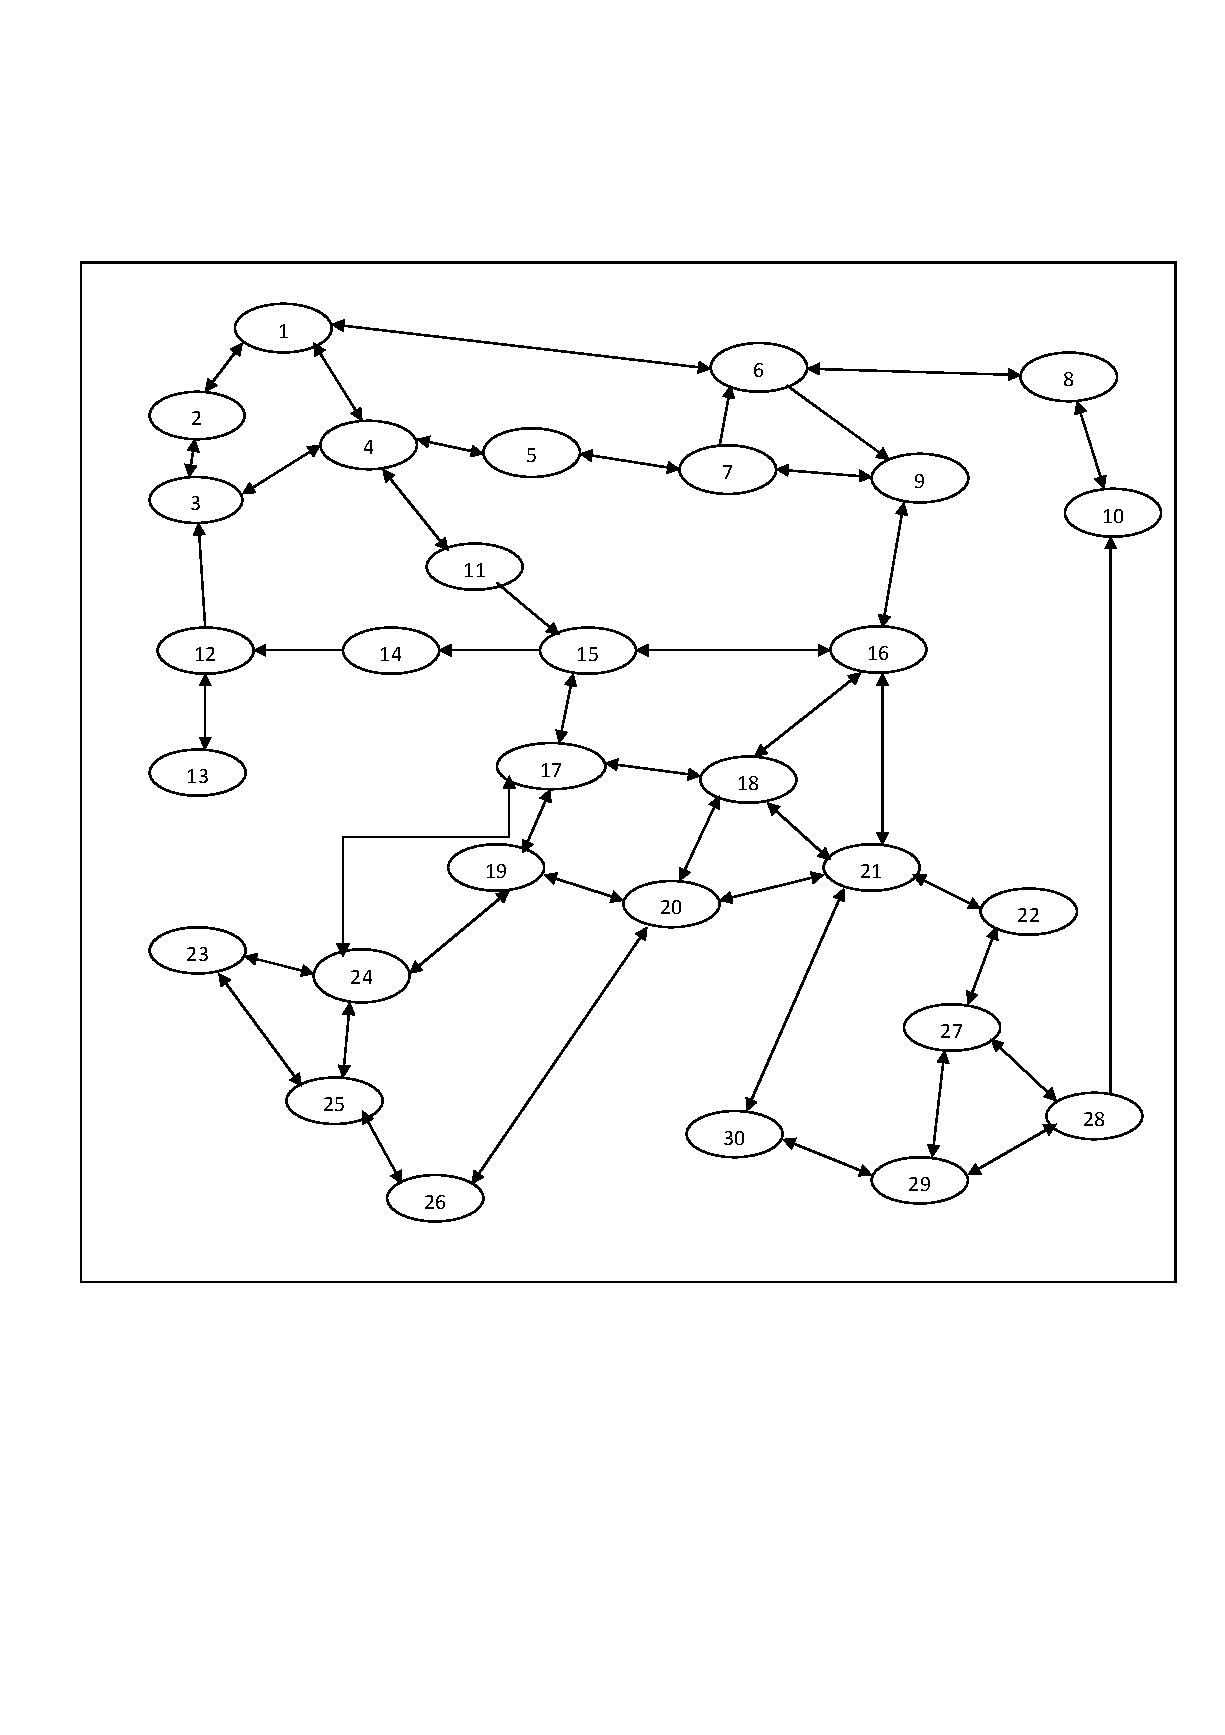
\includegraphics[width=13cm,height=16cm]{flat.eps}
	\vspace{-1.5in}	\caption{Flatgraph}
	\label{fig:flat}
\end{figure}

\hspace*{1cm}Above figure shows the graphical representation of selected area. It is called as flat graph. The flat graph is divided into partitions. In our project we have only 1 partition and 4 fragments of that partition. The figures of fragments are as shown below.\\

\newpage
\begin{figure}[H]
\vspace{-1.2in}
	\centering
		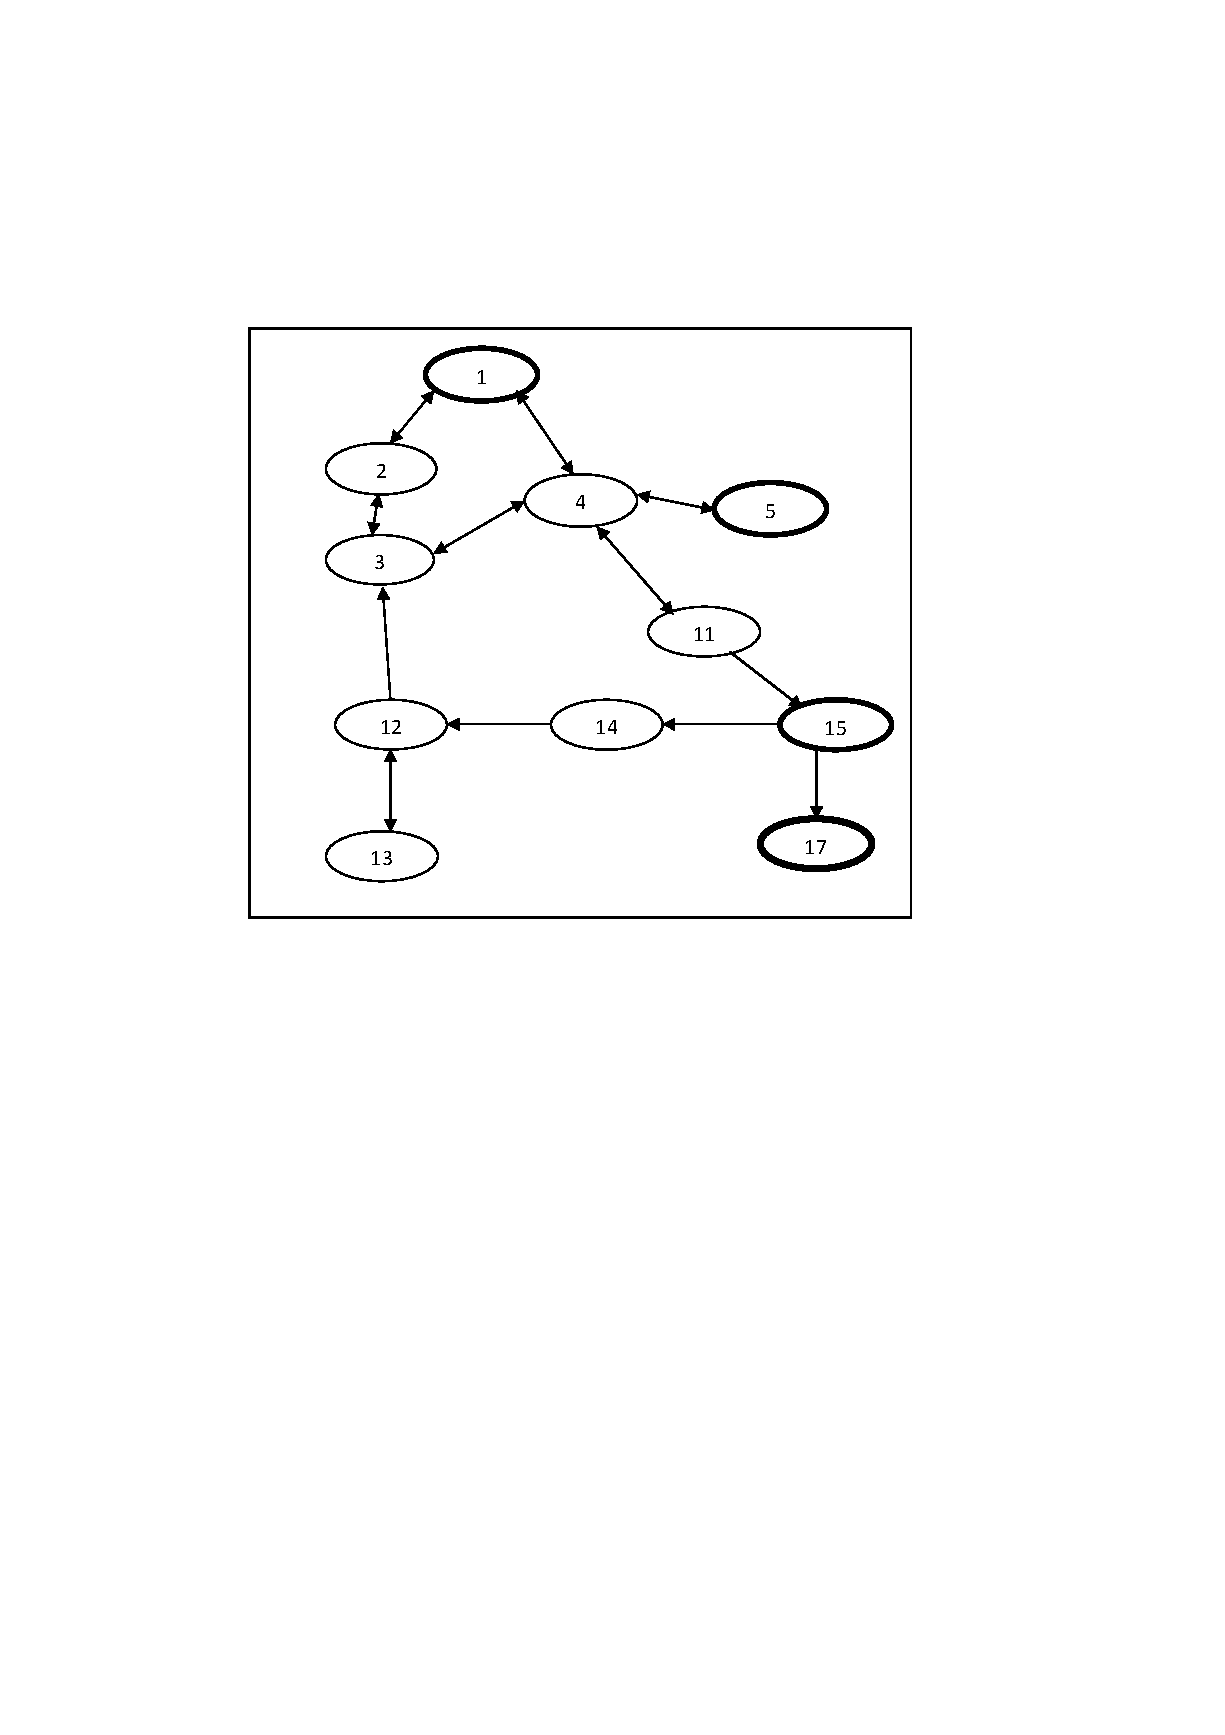
\includegraphics[width=10cm,height=13cm]{frag1.eps}
	\vspace{-1.5in}	\caption{Fragment1}
	\label{fig:frag1}
\end{figure}

\begin{figure}[H]
\vspace{-1.1in}
	\centering
		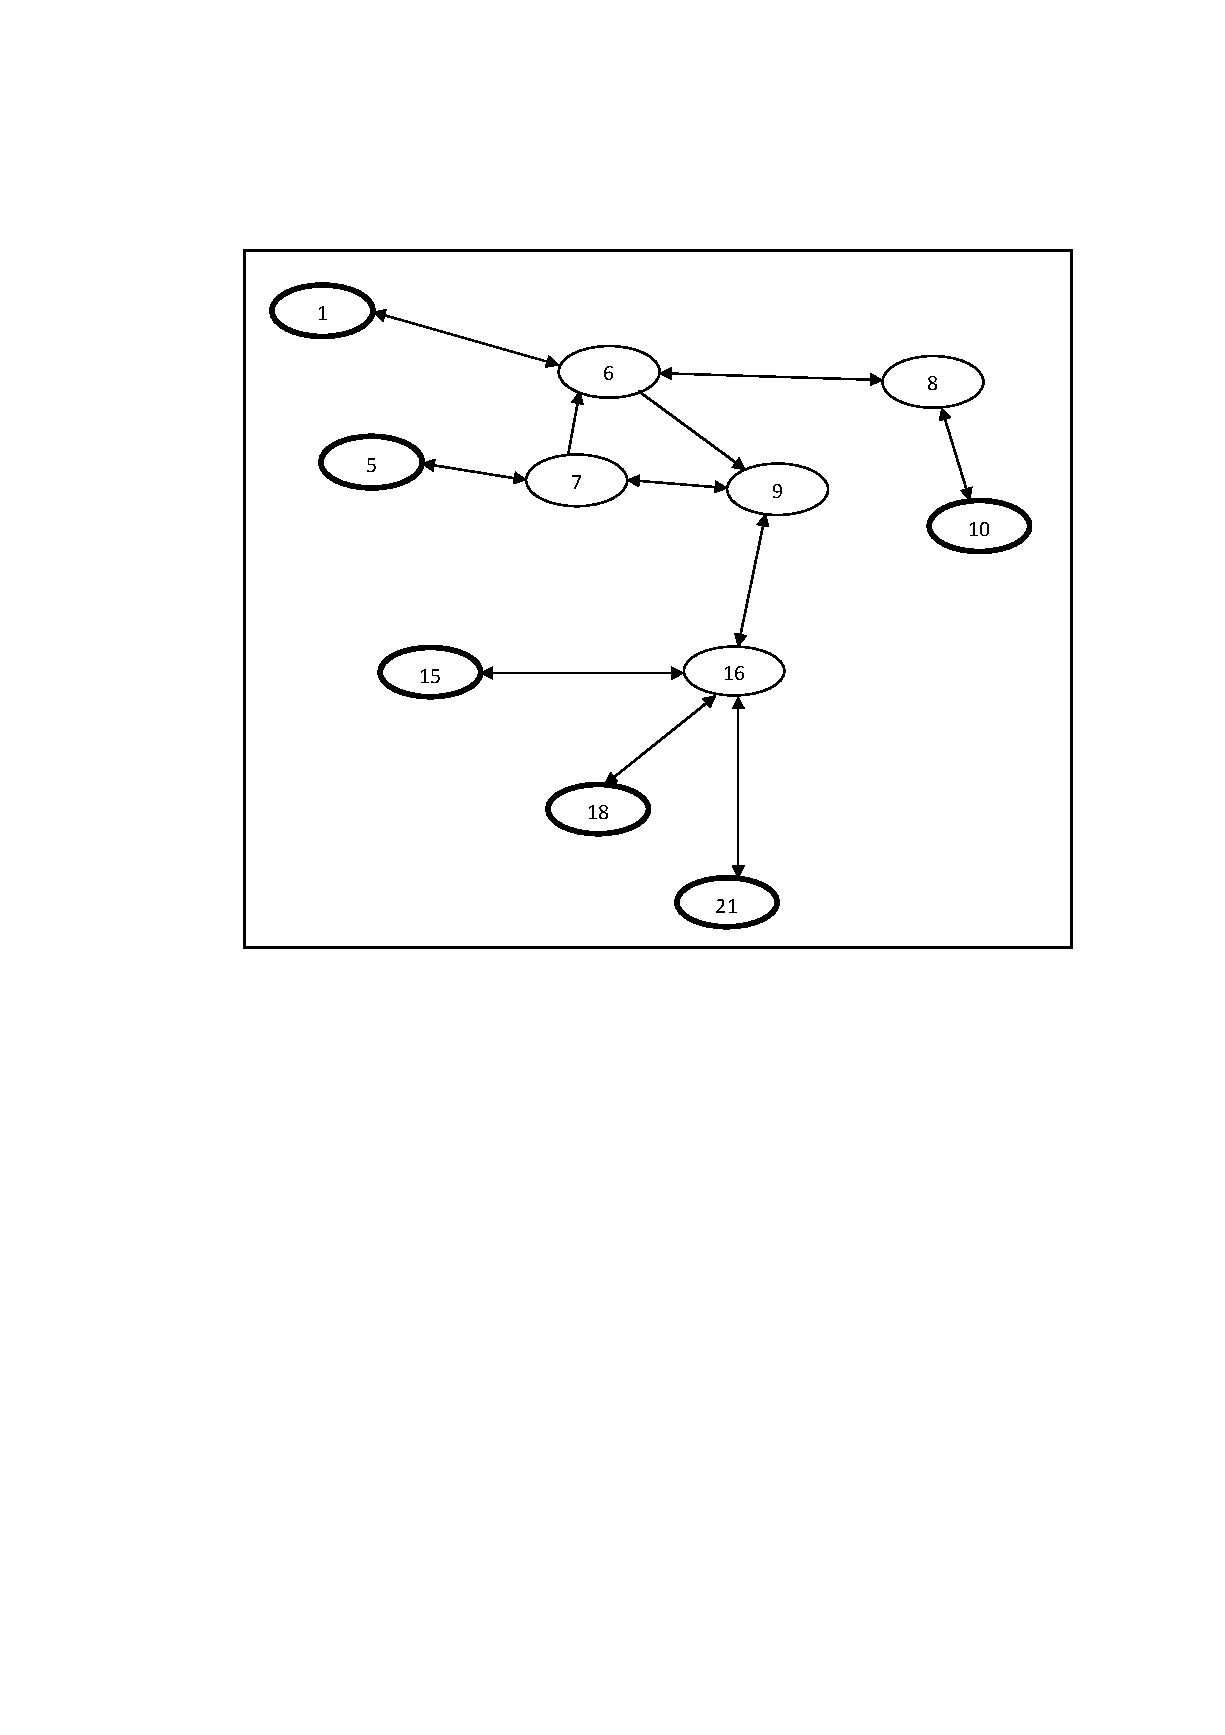
\includegraphics[width=10cm,height=13cm]{frag2.eps}
	\vspace{-1.5in}	\caption{Fragment2}
	\label{fig:frag2}
\end{figure}
\newpage

\begin{figure}[H]
\vspace{-1.4in}
	\centering
		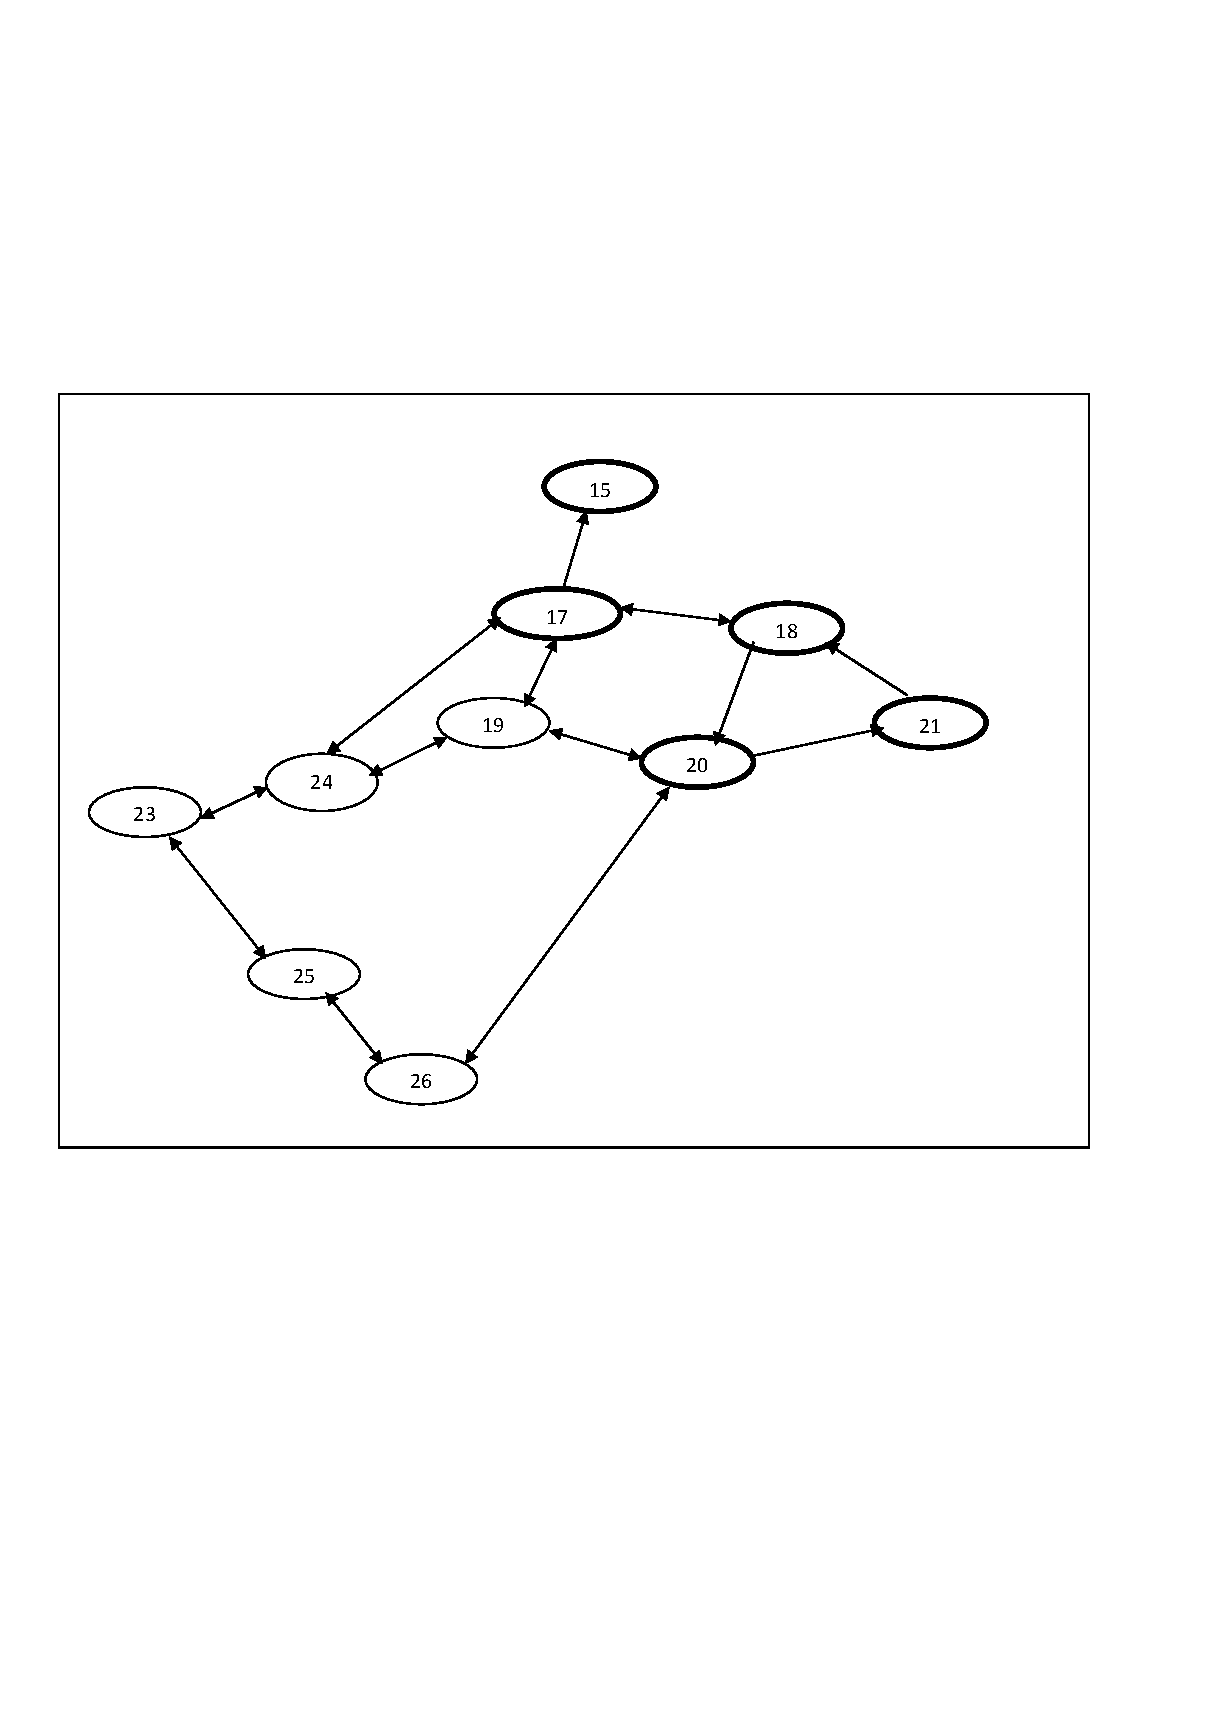
\includegraphics[width=10cm,height=13cm]{frag3.eps}
	\vspace{-1.5in}	\caption{Fragment3}
	\label{fig:frag3}
\end{figure}

\begin{figure}[H]
\vspace{-1.2in}	
	\centering
		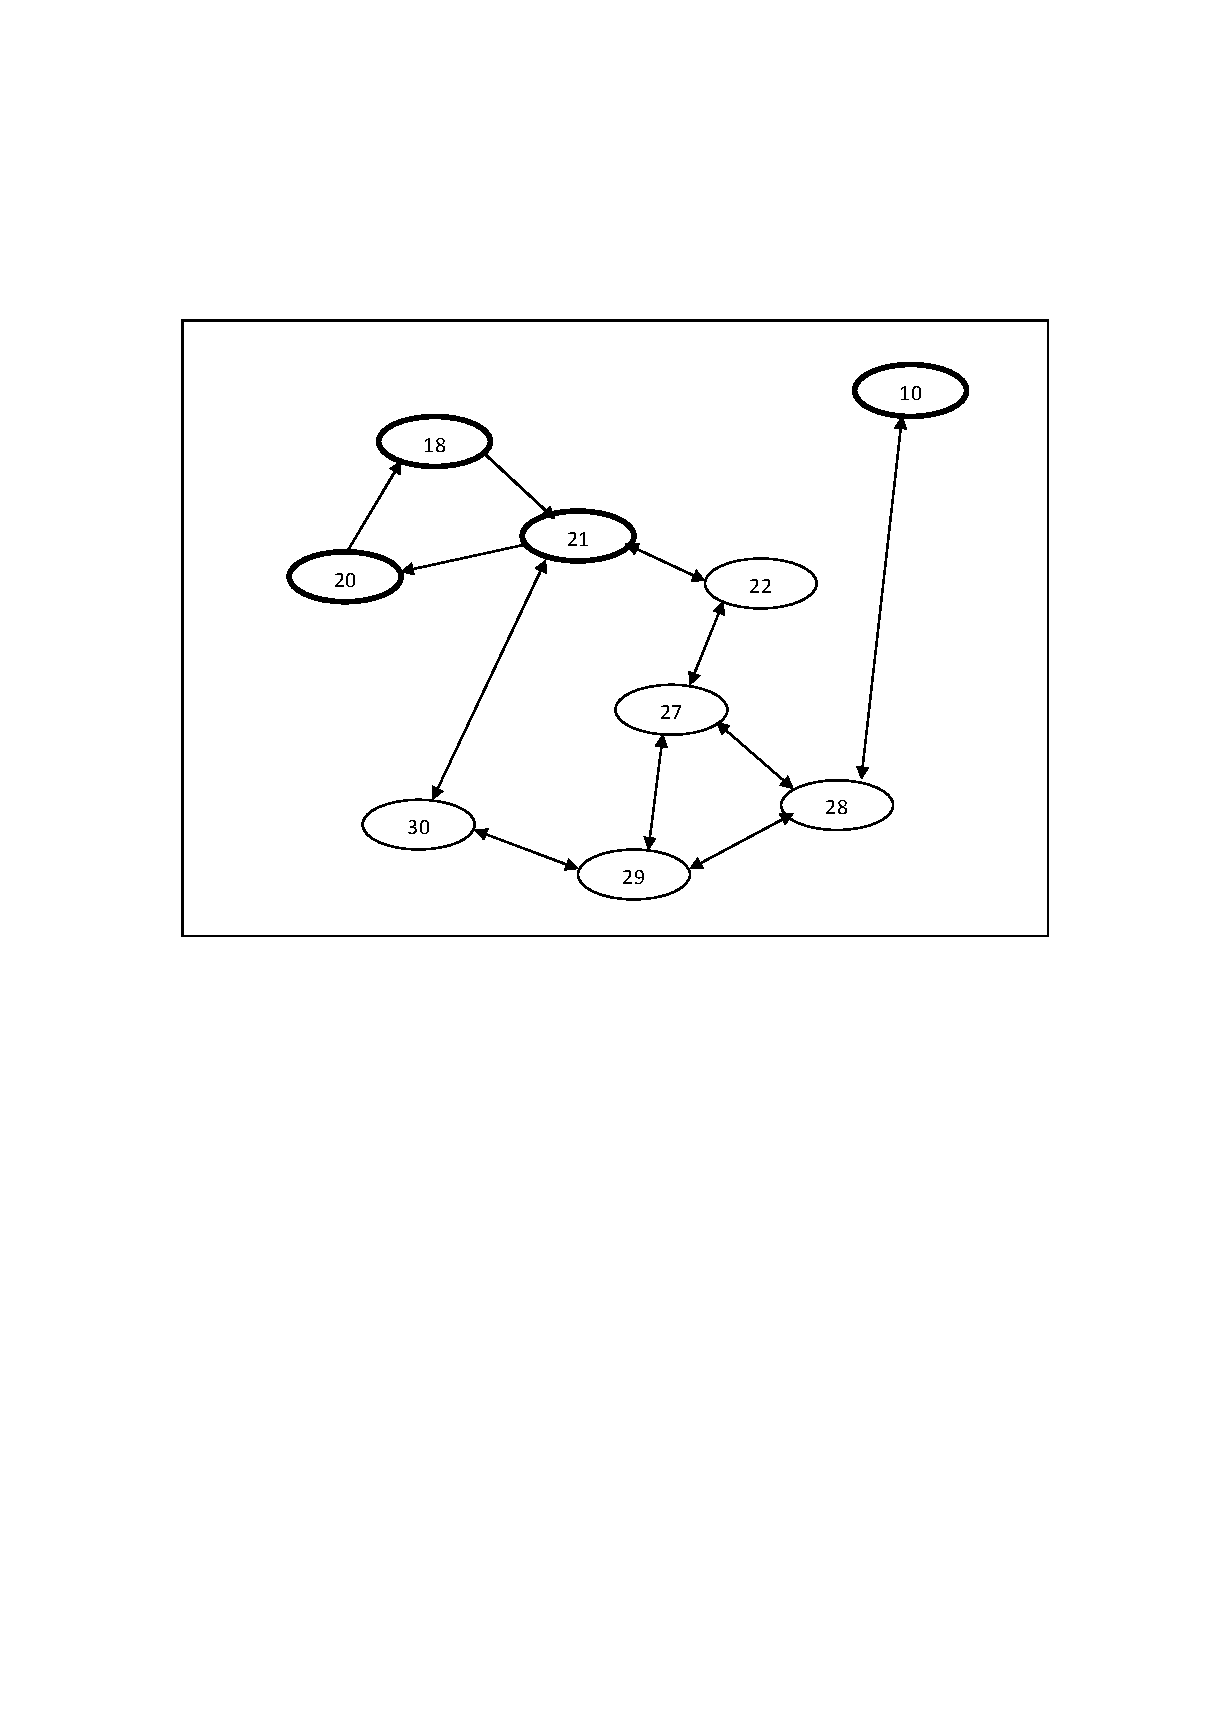
\includegraphics[width=10cm,height=13cm]{frag4.eps}
	\vspace{-1.5in}	\caption{Fragment4}
	\label{fig:frag4}
\end{figure}

\hspace*{1cm}The nodes which are highlighted are border nodes and remaining are local nodes. First we divide the flat graph into no. of small graphs and then by taking a border nodes we create a super graph, which is used to find the optimal path between source and destination. Thus we create a hierarchy of graph. \\

\newpage
\section{\normalsize LITERATURE SURVEY}
%\justifying

\hspace{1cm}Dijikstra algorithm is used to compute the shortest path between two nodes. It calculates the path on demand. It does not precompute the path.  It does not use the concept of fragments. It does not guarantee the optimal solution. It can not handle the large graphs. Thus it is not efficient algorithm for shortest path finding.
\\
\hspace*{1cm}Transitive closure algorithm[2,3] precomputes the paths between source and destination. It does not use fragment also it does not guarantee optimality of a solution.  Theoretically it can handle the huge graph but while much research has been conducted by both the theory and database communities on path finding, many suggested transitive closure algorithms do not effectively handle path computation on large graphs in real-time application domains such as ITS (Intelligent Transportation Systems) systems. With new computer architectures and networks, the traditional algorithms were adapted to parallel and distributed transitive closure algorithms[5].\\
\hspace*{1cm}As an alternative approach, precompute all-pair shortest paths and store them in an encoded path view structure. Queries can be efficiently answered by performing simple lookups on the precomputed path view. This approach is a trade-off between computing paths from scratch and precomputing all paths. While this approach has been proven to be promising for relatively small map data sets, it was determined that it exceeds the memory capacity of typical computer systems for large graphs (e.g., graphs of 3,600 nodes or larger) and the performance of computing the path view deteriorates quickly (e.g., it takes 4 minutes for a graph with 3,600 nodes on a Sun SPARC-20).\\
\hspace*{1cm}The hierarchical abstraction has been proposed by some researchers to overcome this problem[5]. for example divided a relation into fragments and introduced the notion of high-speed fragment. Unfortunately, the formation of high speed fragments are very sensitive to the update of the underlying base relation. Therefore the authors recommended this approach only for rather stable base relations. Some researches have presented a hierarchical graph model which classifies links according to road types and pushes up high speed roads such as highways to the next higher level of hierarchy. However, the paths retrieved from such hierarchical graphs are not guaranteed to be optimal.\\
\hspace*{1cm}A hierarchical A* algorithm for road navigation systems, which while more efficient than flat A* does not guarantee optimality either. It can handle large graph. It uses both the techniques of precomputation and on demand computation.\\
\hspace*{1cm} Similarly, some other researchers proposed another hierarchical multigraph model by dividing graph into subgraphs and pushing up the precomputed paths as well as links between the boundary nodes. The paper did not discuss how the optimality can be achieved. Hierarchical graph refreshing essential for road navigation to reflect the dynamic traffic condition was also not handled.\\


\section{\normalsize PROBLEM DEFINITION}
\subsection{Software Requirement Specification}
\textbf{Problem Statement:}\\
%\justifying
\hspace*{1cm}To find an optimal path for an individual to travel in an alien place such that intermediate nodes are revealed. The capability of computing path queries is an essential feature for advanced database applications. Our goal is to explore solutions for path finding in general with particular focus on addressing the problems inherent to navigation systems applications.
\vspace{.2in}\\
\textbf{Intended Audience and Reading Suggestions:}\\
%\justifying
\hspace*{1cm}This SRS is used by developers, project managers, marketing staff, users, testers and documentation writers for different purposes like developer refers this SRS for coding, testers to build test plans, marketing staff for deciding marketing strategies. This SRS also contains scope of the project, references, project features etc.
\vspace{.2in}\\
\textbf{Project Scope:}\\
%\justifying
\hspace*{1cm}This system is developed under windows environment in JAVA�.. Simple database are used and also simple program files are used. There are separate files for each transaction. 
\\
\hspace*{1cm}1.	We are concerned with providing answers to path queries issued by a potentially large number of concurrent requests (e.g., during peak rush hour periods).
\\ \hspace*{1cm}2.	Our solution must handle the dynamic nature of transportation networks, i.e., it must provide up-to-date query results even when the underlying transportation networks change frequently.  
\\ \hspace*{1cm}3.	Our solution must provide response at a near real-time level of performance (i.e., within seconds). 
\\ \hspace*{1cm}4.  Based on the requirements of instruction based navigation systems, we are interested in efficiently determining the next link for the desired path rather than necessarily retrieving the complete path all at once.
\vspace{.2in}\\
\textbf{Product Perspective:}\\
%\justifying
\hspace*{1cm}The product is standalone application and It is neither a distributed nor a client-server system. 
\vspace{.2in}\\
\textbf{Product Features:}\\
%\justifying
\hspace*{1cm}
1.	Optimal Path
\\
\hspace*{1cm}2.	Intermediate nodes
\vspace{.2in}\\
\textbf{User Classes and Characteristics:}\\
%\justifying
\hspace*{1cm}1.	User-requires some knowledge about computers. How to use the system.
\\	
\hspace*{1cm}2.	Employee should be well trained to handle the application. He/she must know all the features and functions of this software,so he can update the database.
\vspace{.2in}\\
\textbf{Operating Environment :}\\
%\justifying
\hspace*{1cm}Windows operating system 
\vspace{.2in}\\
\textbf{Design and Implementation Constraints:}\\
\hspace*{1cm}Databases to be used : Oracle 10g\\
\hspace*{1cm}Language requirements : JAVA
\vspace{.2in}\\
\textbf{User Documentation:}\\
%\justifying
\hspace*{1cm}User manuals, help ,CD and tutorials
\vspace{.2in}\\
\textbf{Assumptions and Dependencies:}\\
%\justifying
\hspace*{1cm}The graph of interconnected places within city is predefined .This graph can be modified depending on requirement. The computer system on which our product is installed should have sufficient resources to store this information.\\
\hspace*{1cm}We assume that our product does not provide networking capabilities. It is a standalone application.

\vspace{.15cm}
\newpage
\subsection{Project Plan}


%\end{flushleft}
%\begin{center}
 %   \begin{tabular}{| l | p{8cm} | l | l | l |}
 %   \hline
 %  \textbf{ No.}  &	\textbf{Task} &	\textbf{Starting} &	\textbf{Finish} & \textbf{No.of days}\\ %\hline
%   1 &	Project selection &	16/07/2011 &	11/08/2011 & 26 \\ \hline
%   2 & Discuss about various projects &	16/07/2011 & 23/07/2011 & 7 \\ \hline
%   3 &	Project topic searching &	23/07/2011 &	02/08/2011 &	10\\ \hline
%4 &	“Hierarchical Optimization of Optimal Path Finding for
%Transportation Applications” as a project. & 03/08/2011 & 03/08/2011 &	1\\ \hline
%5 & Synopsis creation &  04/08/2011	& 11/08/2011 &	8\\ \hline
%6 & 1st Review &	24/08/2011	& 24/08/2011 &	1\\ \hline
%7 & Approval of project	& 24/08/2011 &	24/08/2011 &	1\\ \hline
%8 & Information gathering &	25/08/2011	& 19/09/2011 &	25\\ \hline
%9	& Collecting required  documents &	25/08/2011	&      2/09/2011 &	8\\ \hline
%10 &	Study of IEEE papers and references &	30/08/2011 &	17/09/2011 &	18\\ \hline
%11	& Estimate resources required	& 12/09/2011 &	19/09/2011	& 8\\ \hline
%12	 & Documentation and designing &	17/09/2011	& 4/10/2011 &	17\\ \hline
%13 &	UML ,DFD , Activity Diagrams &	17/09/2011	& 4/10/2011	& 17\\ \hline
%14	& 2nd  Review & 	05/10/2011	 & 05/10/2011 &	1\\ \hline
%15 &	SRS generation &	05/10/2011 &	06/10/2011 &	2\\ \hline
%16	& Partial Report generation &	05/10/2011	& 07/10/2011 &	3\\ \hline
%    \end{tabular}
%\end{center}

